\documentclass[a4paper,twoside]{article}
\usepackage{enumerate}
%\usepackage{enumitem}
\usepackage{graphicx}
\graphicspath{{Figuras/}}
\usepackage{color}
\usepackage[cmex10]{amsmath}
\usepackage{array}
\usepackage{float}
\usepackage{multicol}
\usepackage[utf8]{inputenc} 
\usepackage[T1]{fontenc}
\usepackage[french]{babel}
%\usepackage[font=normalsize,format=plain,labelfont=bf,up,textfont=up,figurename=Figura,tablename=Tabela]{caption}
\usepackage[tablename=Tableau]{caption}
\usepackage{subcaption}
\usepackage[top=1in, bottom=1in, left=1.25in, right=1.25in]{geometry}
\usepackage{indentfirst}
\usepackage{fancyhdr}
% Font packages
\usepackage{amssymb}
\usepackage{amsfonts}
\usepackage{pgfgantt}
\usepackage{steinmetz}
\usepackage{rotating}
% Nice extra font package, e.g. \mathds{1}
\usepackage{dsfont}
\usepackage{color}
\usepackage{blindtext}
% Use multiple rows when writing tables
\usepackage{multirow}
\usepackage{booktabs}
\usepackage{bm}
\usepackage{bigstrut}
% Uncomment next line to make footnots per page
\usepackage{perpage}
% Uncoment next group of lines to create the table of contents for the PDF
\usepackage{hyperref}
\usepackage[toc,page]{appendix}
\usepackage{listings}
\usepackage{currfile}

\definecolor{darkblue}{rgb}{0,0,0.5}
\definecolor{darkblue}{rgb}{0,0,0.5}
\renewcommand{\title}{Étude des régulations en tension des réseaux de distribution}
\newcommand{\subtitle}{Rapport d'activité de Stage 2A}

\hypersetup{
    pdftitle={\title},
    pdfauthor={Rafael Accacio Nogueira},
    bookmarksnumbered=true,     
    bookmarksopen=true,         
    bookmarksopenlevel=1,       
    colorlinks=true,
    linkcolor=black,
    filecolor=darkblue,  
    urlcolor=darkblue,  
    citecolor=darkblue,              
    pdfstartview=Fit,          
    pdfpagemode=UseOutlines,    % this is the option you were lookin for
    pdfpagelayout=TwoPageRight
}
\let\oldcontentsline\contentsline%
\renewcommand\contentsline[4]{%
    \oldcontentsline{#1}{\smash{\raisebox{1em}{\hypertarget{toc#4}{}}}#2}{#3}{#4}}

\newcommand\mysection[1]{\section[#1]{\protect\hyperlink{tocsection.\thesection}{#1}}\label{#1}}
\newcommand\mysubsection[1]{\subsection[#1]{\protect\hyperlink{tocsection.\thesection}{#1}}\label{#1}}
\newcommand\mysubsubsection[1]{\subsubsection[#1]{\protect\hyperlink{tocsection.\thesection}{#1}}\label{#1}}

\newcommand{\conteudo}{\tableofcontents\label{tocsection}}


\pagestyle{fancy}
\newif\ifdebug
\newcommand{\draft}{\debugtrue}
\newcommand{\final}{\debugfalse}
\newcommand\todo[1]{\ifdebug {\color{red}#1}\else \PackageError{}{FORGOT TO DO SOMETHING}{}\fi}
\newcommand\doing[1]{\ifdebug {\color{blue}#1}\fi}
\newcommand\warning[1]{\ifdebug {\color{red}#1}\fi}


\fancyhead[CO]{\title}
\fancyhead[CE]{\subtitle}
%\fancyhead[RE]{\rightmark}
\fancyhead[L]{\warning{DRAFT}}
\fancyhead[R]{\warning{DEBUG ON}}

\fancyfoot[L]{\warning{TURN DEBUG OFF}}
\fancyfoot[R]{\warning{DRAFT}}

\fancyfoot[C]{\thepage}

\allowdisplaybreaks

\usepackage{chngcntr}
\counterwithin{figure}{section}


\newcommand{\figplaceholder}[1]{\ifdebug
	\begin{figure}[H]
		\begin{center}	
			\rule{8cm}{8cm}
			\caption{\color{red}placeholder}
			\label{fig:#1}
		\end{center}
	\end{figure}
\else
\PackageError{}{NO FIGURE}{}
\fi
}


\usepackage[acronym]{glossaries}\makeglossaries
\newcommand{\acr}[3]{\newacronym{#1}{#2}{#3}}
\newcommand{\symbl}[3]{\newglossaryentry{#1}{name = #2,	description = #3,}}





\debugtrue


\makeindex



\begin{document}

\maketitle

\mysection{Introduction}
Ici un petit résumé des choses faites et les résultats obtenus pendant le stage, du début au 28 de août.
\mysection{Division du travail}
Le travail a été divisé en plusieurs parties a fin de faciliter l'acquisition des résultats.

\mysubsection{Première Partie}
Ce partie consistait de lire l'article de WAN Yidong \cite{yidong} et des extraits de la thèse de Marjorie  Cosson \cite{cosson:tel-01374469}, pour comprendre le problème et ses implications. Autres lectures supplémentaire ont été faites, \cite{farina2015model} et \cite{mariani2013controllo}.

\mysubsection{Deuxième Partie}
Après la lecture des documents commençait l'étude et pris en main du logiciel DIgSILENT PowerFactory, en lisant et regardant les tutoriels a l'internet, en faisant quelques petits exemples du logiciel a fin d'apprendre les outils nécessaires pour faire les tests proposés et après la montage de la modèle du réseaux dans le PowerFactory, le diagramme montré dans la figure \ref{fig:Diagramme_du_reseaux} 

\mysubsection{Troisième Partie}
Pendant ce partie diverses scripts ont été crées en utilisant les langages MATLAB et Python:
\begin{itemize}
\item Pour charger les valeurs de puissance des charges.
\item Pour charger les valeurs de puissance des générateurs.
\item Pour calculer les gains entre les bus et les générateurs.
\item Pour faire des matrices de gains.
\item Pour créer des événements de charges et générateurs, faire des simulations et prendre les résultats en graphiques.
\end{itemize}

\mysubsection{Quatrième Partie}
Pendant la quatrième partie la interface entre le PowerFactory et MATLAB a été requise a fin de créer une modèle de régulateur au simulink et utiliser dans le PowerFactory. Le Régulateur a été déjà crée et quelques configurations dans le PowerFactory sont manquantes.


\mysubsection{Cinquième Partie}
La cinquième partie est la élaboration des rapports de conclusion du stage, pour la CentraleSupélec et l'IETR et ce document.



\begin{figure}[H]
	\begin{center}	
		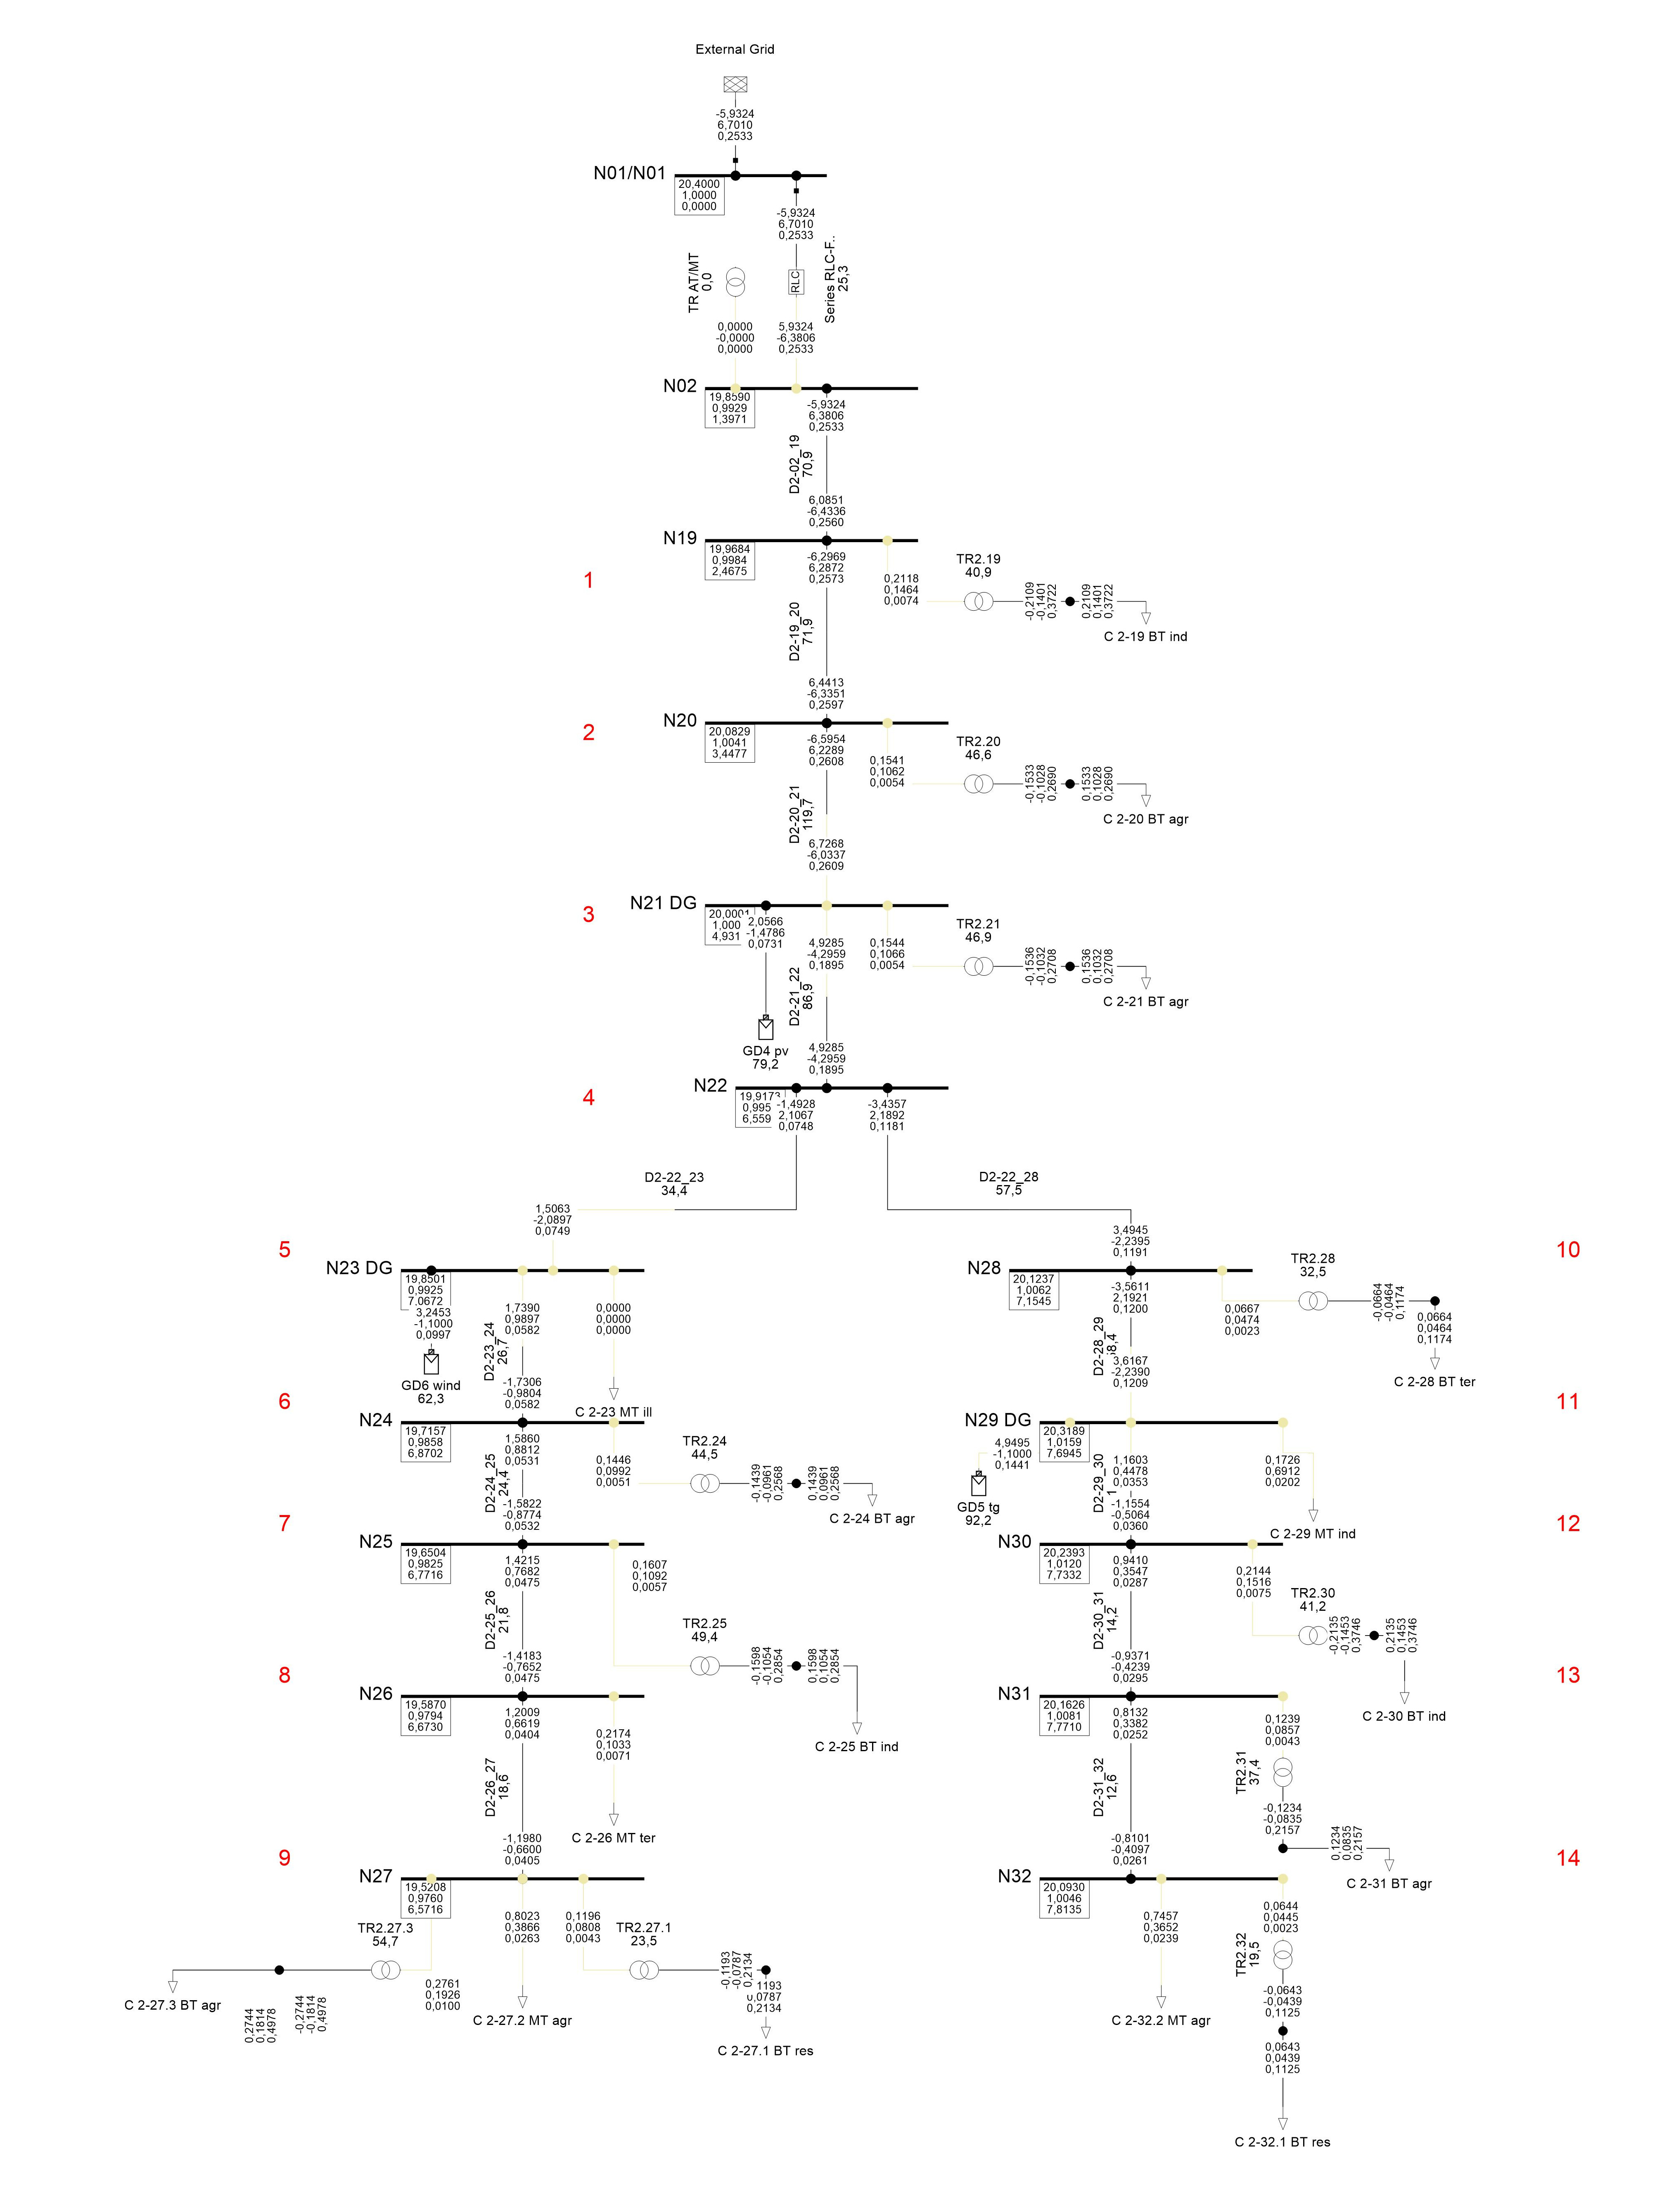
\includegraphics[width=\textwidth]{Division_du_travail/Diagramme_du_reseaux.jpg}
		\caption{Diagramme du reseaux}
		\label{fig:Diagramme_du_reseaux}
	\end{center}
\end{figure}
\pagebreak

\mysection{Résultats}
\mysubsection{Scripts}
En dessous les résultats provenus des scripts crées dans la troisième partie du projet. 
\paragraph{gain\_calc-load2bus\\\\}
Ce script calcule le gain entre la puissance reactive des charges et la tension des bus aux lesquels elles sont connectées.

\tiny
\hspace{-70pt}
\begin{tabular}{ccccccccccccccccc}
	%	1&2&3&4&5&6&7&8&9&10&11&12&13&14&15&16&17\\
	0e+0&-9.3e-5&-1.2e-4&-1.1e-4&-1.1e-4&-1.1e-4&-1.1e-4&-1.2e-4&-1.2e-4&-1.2e-4&-1.2e-4&-1.1e-4&-1.1e-4&-1.1e-4&-1.1e-4&-1.1e-4&-1.1e-4\\
	0e+0&-8.9e-5&-1.1e-4&-1.3e-4&-1.3e-4&-1.3e-4&-1.3e-4&-1.3e-4&-1.3e-4&-1.3e-4&-1.3e-4&-1.3e-4&-1.3e-4&-1.3e-4&-1.3e-4&-1.3e-4&-1.3e-4\\
	0e+0&-9.1e-5&-1.1e-4&-1.3e-4&-1.8e-4&-1.8e-4&-1.8e-4&-1.8e-4&-1.8e-4&-1.8e-4&-1.8e-4&-1.8e-4&-1.8e-4&-1.8e-4&-1.8e-4&-1.8e-4&-1.8e-4\\
	0e+0&-1.2e-4&-1.5e-4&-1.8e-4&-2.5e-4&-3.5e-4&-4.2e-4&-4.2e-4&-4.2e-4&-4.3e-4&-4.3e-4&-3.4e-4&-3.4e-4&-3.4e-4&-3.4e-4&-3.4e-4&-3.4e-4\\
	0e+0&-9.4e-5&-1.2e-4&-1.4e-4&-1.9e-4&-2.7e-4&-3.3e-4&-3.9e-4&-3.9e-4&-3.9e-4&-3.9e-4&-2.6e-4&-2.6e-4&-2.6e-4&-2.6e-4&-2.6e-4&-2.6e-4\\
	0e+0&-9.5e-5&-1.2e-4&-1.4e-4&-1.9e-4&-2.7e-4&-3.3e-4&-4.0e-4&-4.3e-4&-4.3e-4&-4.3e-4&-2.7e-4&-2.6e-4&-2.6e-4&-2.6e-4&-2.7e-4&-2.7e-4\\
	0e+0&-9.3e-5&-1.2e-4&-1.4e-4&-1.9e-4&-2.6e-4&-3.2e-4&-3.9e-4&-4.2e-4&-4.6e-4&-4.6e-4&-2.6e-4&-2.6e-4&-2.6e-4&-2.6e-4&-2.6e-4&-2.6e-4\\
	0e+0&0e+0&0e+0&0e+0&0e+0&0e+0&0e+0&0e+0&0e+0&0e+0&0e+0&0e+0&0e+0&0e+0&0e+0&0e+0&0e+0\\
	0e+0&0e+0&0e+0&0e+0&0e+0&0e+0&0e+0&0e+0&0e+0&0e+0&0e+0&0e+0&0e+0&0e+0&0e+0&0e+0&0e+0\\
	0e+0&-9.7e-5&-1.2e-4&-1.4e-4&-2.0e-4&-2.7e-4&-3.4e-4&-4.0e-4&-4.4e-4&-4.8e-4&-5.2e-4&-2.7e-4&-2.7e-4&-2.7e-4&-2.7e-4&-2.7e-4&-2.7e-4\\
	0e+0&-9.5e-5&-1.2e-4&-1.4e-4&-1.9e-4&-2.7e-4&-2.7e-4&-2.7e-4&-2.7e-4&-2.7e-4&-2.7e-4&-2.8e-4&-2.8e-4&-2.8e-4&-2.8e-4&-2.8e-4&-2.8e-4\\
	0e+0&-9.1e-5&-1.1e-4&-1.3e-4&-1.9e-4&-2.6e-4&-2.6e-4&-2.6e-4&-2.6e-4&-2.6e-4&-2.6e-4&-2.7e-4&-2.8e-4&-2.8e-4&-2.8e-4&-2.9e-4&-2.9e-4\\
	0e+0&-9.5e-5&-1.2e-4&-1.4e-4&-1.9e-4&-2.7e-4&-2.7e-4&-2.7e-4&-2.7e-4&-2.7e-4&-2.7e-4&-2.9e-4&-3.0e-4&-3.0e-4&-3.1e-4&-3.1e-4&-3.1e-4\\
	0e+0&-9.3e-5&-1.2e-4&-1.4e-4&-1.9e-4&-2.7e-4&-2.7e-4&-2.7e-4&-2.7e-4&-2.7e-4&-2.7e-4&-2.8e-4&-2.9e-4&-2.9e-4&-3.1e-4&-3.2e-4&-3.2e-4\\
	0e+0&0e+0&0e+0&0e+0&0e+0&0e+0&0e+0&0e+0&0e+0&0e+0&0e+0&0e+0&0e+0&0e+0&0e+0&0e+0&0e+0\\
	0e+0&-9.2e-5&-1.2e-4&-1.4e-4&-1.9e-4&-2.6e-4&-2.6e-4&-2.6e-4&-2.6e-4&-2.6e-4&-2.6e-4&-2.8e-4&-2.9e-4&-2.9e-4&-3.0e-4&-3.2e-4&-3.4e-4\\
\end{tabular} 
\normalsize
\paragraph{gain\_calc-generator2bus-test\_1\_-7am\\\\}
Ce script calcule le gain entre la puissance réactive des générateurs et la tension des bus aux lesquels ils sont connectés, avec les valeurs de charges de 7 heures et en faisant la puissance réactive des générateurs diminuer en 20\%.

\begin{tabular}{ccc}
	1.7e-4&1.7e-4&1.7e-4\\
	1.7e-4&2.5e-4&2.7e-4\\
	1.7e-4&3.1e-4&2.4e-4\\
\end{tabular}

\paragraph{gain\_calc-generator2bus-test\_1\_-1pm\\\\}
Ce script calcule le gain entre la puissance réactive des générateurs et la tension des bus aux lesquels ils sont connectés, avec les valeurs de charges de 13 heures et en faisant la puissance réactive des générateurs diminuer en 20\%.

\begin{tabular}{ccc}
	1.7e-4&1.7e-4&1.6e-4\\
	1.7e-4&2.4e-4&2.7e-4\\
	1.7e-4&3.0e-4&2.4e-4\\
\end{tabular}
\paragraph{gain\_calc-generator2bus-test\_2\\\\}
Ce script calcule le gain entre la puissance réactive des générateurs et la tension des bus aux lesquels ils sont connectés, avec les valeurs de charges de 13 heures et en faisant la puissance réactive des générateurs augmenter en 20\%.

\begin{tabular}{ccc}
	
	1.8e-4&1.8e-4&1.7e-4\\
	
	1.8e-4&2.5e-4&2.8e-4\\
	
	1.8e-4&3.1e-4&2.5e-4\\
\end{tabular}

\paragraph{teste\_simul\\\\}
Ce script crée un événement des changement de valeur de puissance active de la charge C 2-29 MT ind en augmentant sa valeur en 100\% par un période de temps et après prend les valeurs de puissance active et réactive des cette même charge et la tension des bus N21 N23 et N29 ( où les générateurs sont connectés ) pendant le temps de la simulation et en exportant en un fichier $ \verb|.csv| $ pour faire des graphiques, figures \ref{fig:Puissance_Active_et_Reactive_de_la_Charge_C2_29_MT} et \ref{fig:Tension_des_Bus_N21_N23_et_N29}.
\begin{figure}[H]
	\begin{center}	
		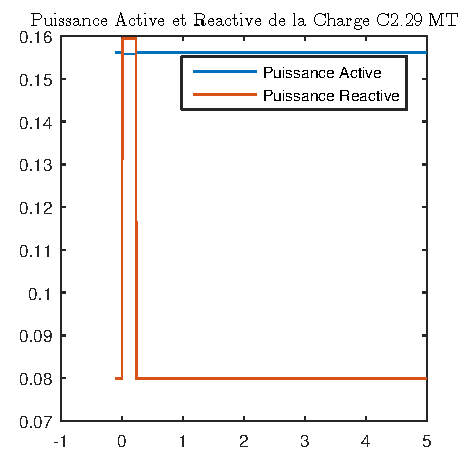
\includegraphics[width=8cm]{Resultats/Puissance_Active_et_Reactive_de_la_Charge_C2_29_MT.pdf}
		\caption{Puissance Active et Reactive de la Charge C2 29 MT}
		\label{fig:Puissance_Active_et_Reactive_de_la_Charge_C2_29_MT}
	\end{center}
\end{figure}

\begin{figure}[H]
	\begin{center}	
		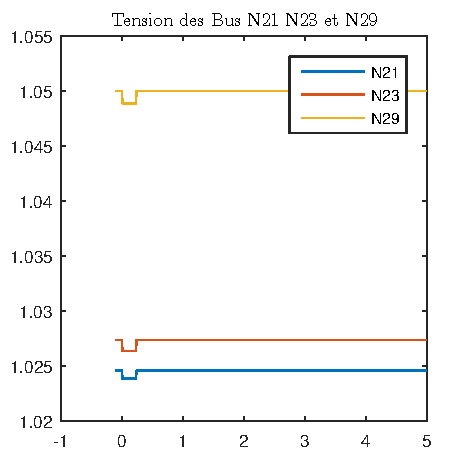
\includegraphics[width=8cm]{Resultats/Tension_des_Bus_N21_N23_et_N29.pdf}
		\caption{Tension des Bus N21 N23 et N29 en p.u.}
		\label{fig:Tension_des_Bus_N21_N23_et_N29}
	\end{center}
\end{figure}

\mysection{Conclusions}
Ces résultats sont les données obtenus par le travail, mais ses respectives conséquences n'ont pas été discutés. Donc il faut faire des discussion e prendre conclusions a partir de la observation des données. Il faut aussi réussir la communication entre MATLAB et PowerFactory et développer le régulateur et comparer avec les données de \cite{cosson:tel-01374469}. Et au but terminer la rédaction des Rapports en donnant un aperçu total de tout ces résultats, discussions e conclusions.



\bibliographystyle{plain}
\bibliography{bibliografia}
\end{document}